\documentclass[12pt]{article}

\usepackage[a4paper,scale=0.8]{geometry}
\usepackage[english]{babel} % needed for English texts
\usepackage[utf8]{inputenc} % unicode encoding
\usepackage{amsmath,amssymb,amsfonts,amsthm}
\usepackage{stmaryrd}
\usepackage{hyperref}  % automagically makes clickable references, table of contents
\usepackage{enumerate}
\usepackage{lipsum}
\usepackage{titlesec}
\usepackage{graphicx}

\usepackage{tikz}
\usetikzlibrary{matrix, positioning}
\tikzset{
	edge/.style={thick, ->},
	table nodes/.style={
		rectangle,
		draw=black,
		style=thick,
		align=center,
		minimum height=7mm,
		text depth=0.5ex,
		text height=2ex,
		inner xsep=0pt,
		outer sep=0pt,
		inner sep=0pt
	},
	table/.style={
		matrix of nodes,
		row sep=-0.5pt,
		column sep=-0.5pt,
		nodes={
			table nodes
		}
	}
}


\newtheorem{definition}{Definition}[section] % defines the definition environment
\newtheorem{theorem}{Theorem}[section] % defines the theorem environment
\newtheorem{lemma}{Lemma}[section]
%\newtheorem{proof}{Proof}[section] % defines the proof environment

% Sets and set operation
\newcommand{\R}{\mathbb{R}} % the reals
\newcommand{\Z}{\mathbb{Z}} % the integers
\newcommand{\N}{\mathbb{N}} % the natural numbers
\renewcommand{\O}[1]{\mathcal{O}\l(#1\r)}
%\newcommand{\pot}[1]{\mathcal{P}(#1)} % power set


% Convenience
\renewcommand{\l}{\left} % short left
\renewcommand{\r}{\right} % short right
\newcommand{\pfrac}[2]{\l( \frac{#1}{#2} \r)}
\newcommand{\explain}[1]{\hspace*{2em} \l(\text{\small #1}\r)} % explanation in proof, indented line with smaller text



% change section titles to inline, bold without numbering
\titleformat{\section}[runin]{\bfseries}{\thesection}{1em}{}[.]


\title{Storing a Sparse Table}
\date{Summer Semester 2016}
\author{Simon Feiden\\Supervisor: Daniel Neuen}


\begin{document}


\maketitle
\thispagestyle{empty}

\vspace*{2em}

\begin{center}
	\begin{minipage}[t]{0.8\textwidth}
		\section*{Abstract} % \\[0.4em]
		\input{bounds/abstract.tex}
	\end{minipage}
\end{center}
\newpage



\section*{Introduction}
In this work, we elaborate and explain the techniques presented in \cite{tarjan:storing_sparse_table} to store a map from words to objects with $\O{1}$ lookup and minimised storage needs.
The words are natural numbers in the range $0$ through $N-1$ while the objects can be arbitrary data.
We consider the \emph{static case} where $n$ words are added to the map before any lookups are performed.
In order to apply several optimisations to our storage scheme, we assume that $N$ is bounded by a polynomial in $n$, i.e.~$N \in \O{n^c}$.
This guarantees that the tables we will compress are sparse, but not too sparse.
Use cases are LR parsing and sparse Gaussian elimination which can be implemented using such tables.
In both cases, $c = 2$ giving $N \in \O{n^2}$. \\
First of all, we will introduce \emph{tries} which are a data structure based on trees.
Then, seemingly unrelated, we will present a way to compress tables in three steps using row and column displacements as well as a special indexing scheme.
Finally, we combine both ideas to obtain a way to store a sparse table with good space complexity.



\section*{Tries à la Knuth}
\begin{frame}{Tries --- Overview}
	\begin{itemize}[<+->]
		\itemspacing{20pt}
		\item Tree data structure for integers
		\item Also known as \emph{prefix trees} for strings
		\item Degree $k$ at every node
		\item Usual operations: \code{insert}, \code{lookup}, \code{delete}
		\item Path in trie specified by a single integer
	\end{itemize}
\end{frame}


\newcommand{\trienode}[2]{% node label, options for matrix
	\matrix (n#1) [table, text width=7mm, ampersand replacement=\&, #2]
	{ #1 \& {} \& {} \& {} \& {} \\};
	\node[font=\tiny, anchor=south] at (n#1-1-2.north) {0};
	\node[font=\tiny, anchor=south] at (n#1-1-3.north) {1};
	\node[font=\tiny, anchor=south] at (n#1-1-4.north) {2};
	\node[font=\tiny, anchor=south] at (n#1-1-5.north) {3}
}

\begin{frame}{Examples --- \code{insert}}
	\resizebox{\textwidth}{!}{%
		
		\begin{tikzpicture}[align=center, node distance=2cm]
			\trienode{30}{};
			
			\trienode{33}{below of=n30};
			\draw[edge] (n30-1-3.south) to[out=270, in=90] (n33-1-1.north);
			
			\visible<3->{
				\trienode{24}{left =2cm of n33};
				\draw[edge] (n30-1-2.south) to[out=250, in=70] (n24-1-1.north);
			}
			
			\visible<5->{
				\alert<6-7>{ \trienode{19}{right=2cm of n33}; }
				\draw[edge] (n30-1-5.south) to[out=270, in=90] (n19-1-1.north);
			}
			
			\visible<8->{
				\trienode{47}{below of=n19};
				\draw[edge] (n19-1-4.south) to[out=270, in=90] (n47-1-1.north);
			}
		\end{tikzpicture}
	}
	
	\begin{itemize}
		\item<2-> $24 \divmod (6, 0)$
		\item<4-> $19 \divmod (4, 3)$
		\item<6-> $47 \divmod (11, 3) \uncover<7->{ \divmod (2, 3) }$
	\end{itemize}
	
\end{frame}


\begin{frame}{Examples --- \code{lookup}}
	\resizebox{\textwidth}{!}{%
		
		\begin{tikzpicture}[align=center, node distance=2cm]
		\alert<2,7>{
			\trienode{30}{};
		}
		
		\alert<9>{
			\trienode{33}{below of=n30};
			\draw[edge] (n30-1-3.south) to[out=270, in=90] (n33-1-1.north);
		}
		
		\alert<4>{
			\trienode{24}{left =2cm of n33};
			\draw[edge] (n30-1-2.south) to[out=250, in=70] (n24-1-1.north);
		}
		
		\trienode{19}{right=2cm of n33};
		\draw[edge] (n30-1-5.south) to[out=270, in=90] (n19-1-1.north);
		
		\trienode{47}{below of=n19};
		\draw[edge] (n19-1-4.south) to[out=270, in=90] (n47-1-1.north);
		\end{tikzpicture}
	}
	
	\begin{itemize}
		\item<2-> $24
				\uncover<3->{ \divmod (6, 0) }
				\phantom{mmm}$
				\uncover<5->{ \ding{51} }
				
		\item<6-> $25
				\uncover<8->{ \divmod (6, 1) }
				\uncover<10->{ \divmod (1, 2) }
				\phantom{mmm}$
				\uncover<11>{ \ding{55}}
	\end{itemize}
	
\end{frame}


\begin{frame}{Examples --- \code{delete}}
	\resizebox{\textwidth}{!}{%
		
		\begin{tikzpicture}[align=center, node distance=2cm]
		\trienode{30}{};
		
		\trienode{33}{below of=n30};
		\draw[edge] (n30-1-3.south) to[out=270, in=90] (n33-1-1.north);
		
		\visible<1-2>{
			\alert<2>{
				\trienode{24}{left =2cm of n33};
				\draw[edge] (n30-1-2.south) to[out=250, in=70] (n24-1-1.north);
			}
		}
		
		\visible<-6>{
			\alert<4,6-7>{
				\trienode{19}{right=2cm of n33};
				\draw[edge] (n30-1-5.south) to[out=270, in=90] (n19-1-1.north);
			}
		}
		
		\visible<7->{
			\alert<7->{
					\matrix (n75b) [table, text width=7mm, ampersand replacement=\&, right=2cm of n33]
						{ 75 \& {} \& {} \& {} \& {} \\};
					\node[font=\tiny, anchor=south] at (n75b-1-2.north) {0};
					\node[font=\tiny, anchor=south] at (n75b-1-3.north) {1};
					\node[font=\tiny, anchor=south] at (n75b-1-4.north) {2};
					\node[font=\tiny, anchor=south] at (n75b-1-5.north) {3};
					\draw[edge] (n30-1-5.south) to[out=270, in=90] (n75b-1-1.north);
			}
		}
		
		\trienode{47}{below of=n19};
		\draw[edge] (n19-1-4.south) to[out=270, in=90] (n47-1-1.north);
		
		\visible<1-5>{
			\alert<5> {
				\trienode{75}{below of=n47};
				\draw[edge] (n47-1-2.south) to[out=270, in=90] (n75-1-1.north);
			}
		}
		\end{tikzpicture}
	}
	
	\begin{itemize}
		\item<1-> \code{delete} 24
		\item<4-> \code{delete} 19
	\end{itemize}
\end{frame}

\begin{frame}{Tries --- Analysis}
	\begin{itemize}[<+->]
		\itemspacing{20pt}
		\item Insertion of $n$ values in range $0, \ldots, N - 1$
		\item Longest path is $\O{\log_k N}$
		\item \code{insert}, \code{lookup}, \code{delete} follow a path (to a leaf)
		\item Constant time changes to nodes in \code{insert}, \code{delete}
		\item Worst case $\O{\log_k N}$ for all three methods
	\end{itemize}
\end{frame}



\section*{Displacements}
In this section, we will show how a static table with null entries can be compressed such that almost no null entries must be stored.
The method works only for the static case, which means that all data is added to the table before any of it is looked up.
All tables are basically two-dimensional arrays that have the same number of rows and columns, i.e.\ they are square.
The remaining setup is similar to tries:
We store $n$ integers in the range $0$ through $N - 1$ in the tables.
Since all integers in the range must fit in a table, $N$ is the table size.
The tables are square, so $N$ must be a square and there is an $m$ such that $N = m^2$.
$m$ is then the number of rows and columns.
Further we assume that $n \geq \max(2, m)$.
The cell $(i, j)$ for an integer $k$ can be found by counting rowwise from the top left until $k$ or by the following formula: $i = \l\lfloor \frac{k}{m} \r\rfloor + 1$ and $j = k \operatorname{mod} m + 1$.
The table entry for $k$ contains the information belonging to $k$ if $k$ is present in the table and null otherwise.

\begin{wrapfigure}{r}{0.5\textwidth}
  %\begin{tikzpicture}[align=center, node distance=2cm]
%\matrix (all) [table, text width=7mm]
%{
%	0 & 0 & * & 0 \\
%	* & * & * & 0 \\
%	0 & * & * & 0 \\
%	* & 0 & 0 & * \\
%};

%\matrix (r2) [table, text width=7mm, below of=all]
%	{ * & * & * & 0 \\};
%	
%\matrix (r3) [table, text width=7mm, below of=r2-1-3]
%	{ 0 & * & * & 0 \\};
%	
%\matrix (r4) [table, text width=7mm, below of=r3-1-4]
%	{ * & 0 & 0 & * \\};
%	
%\matrix (r1) [table, text width=7mm, below of=r4-1-3]
%	{ 0 & 0 & * & 0 \\};


\matrix (mx) [%
		matrix of nodes,
		draw = none,
		row sep = 0.7em,
		column sep = 0em
]
{
	$\s$ & $\s$ & $\s$ & 0    & {}   & {}   & {}   & {} & {}   &[1em] $r_2 = 0$ \\
	{}   & {}   & 0    & $\s$ & $\s$ & 0    & {}   & {} & {}   & $r_3 = 2$ \\
	{}   & {}   & {}   & {}   & {}   & $\s$ & 0    & 0  & $\s$ & $r_4 = 5$ \\
	{}   & {}   & {}   & {}   & 0    & 0    & $\s$ & 0  & {}   & $r_1 = 3$ \\
	5    & 6    & 7    & 10   & 11   & 13   & 3    & 0  & 16   & $\phantom{r_1 = } C$ \\
};


\node[draw, fit = (mx-1-1) (mx-1-4)] (1-fit) {};

\node[draw, fit = (mx-2-3) (mx-2-6)] (2-fit) {};

\node[draw, fit = (mx-3-6) (mx-3-9)] (3-fit) {};

\node[draw, fit = (mx-4-5) (mx-4-8)] (4-fit) {};

\node[draw, fit = (mx-5-1) (mx-5-9)] (C-fit) {};


\end{tikzpicture}
  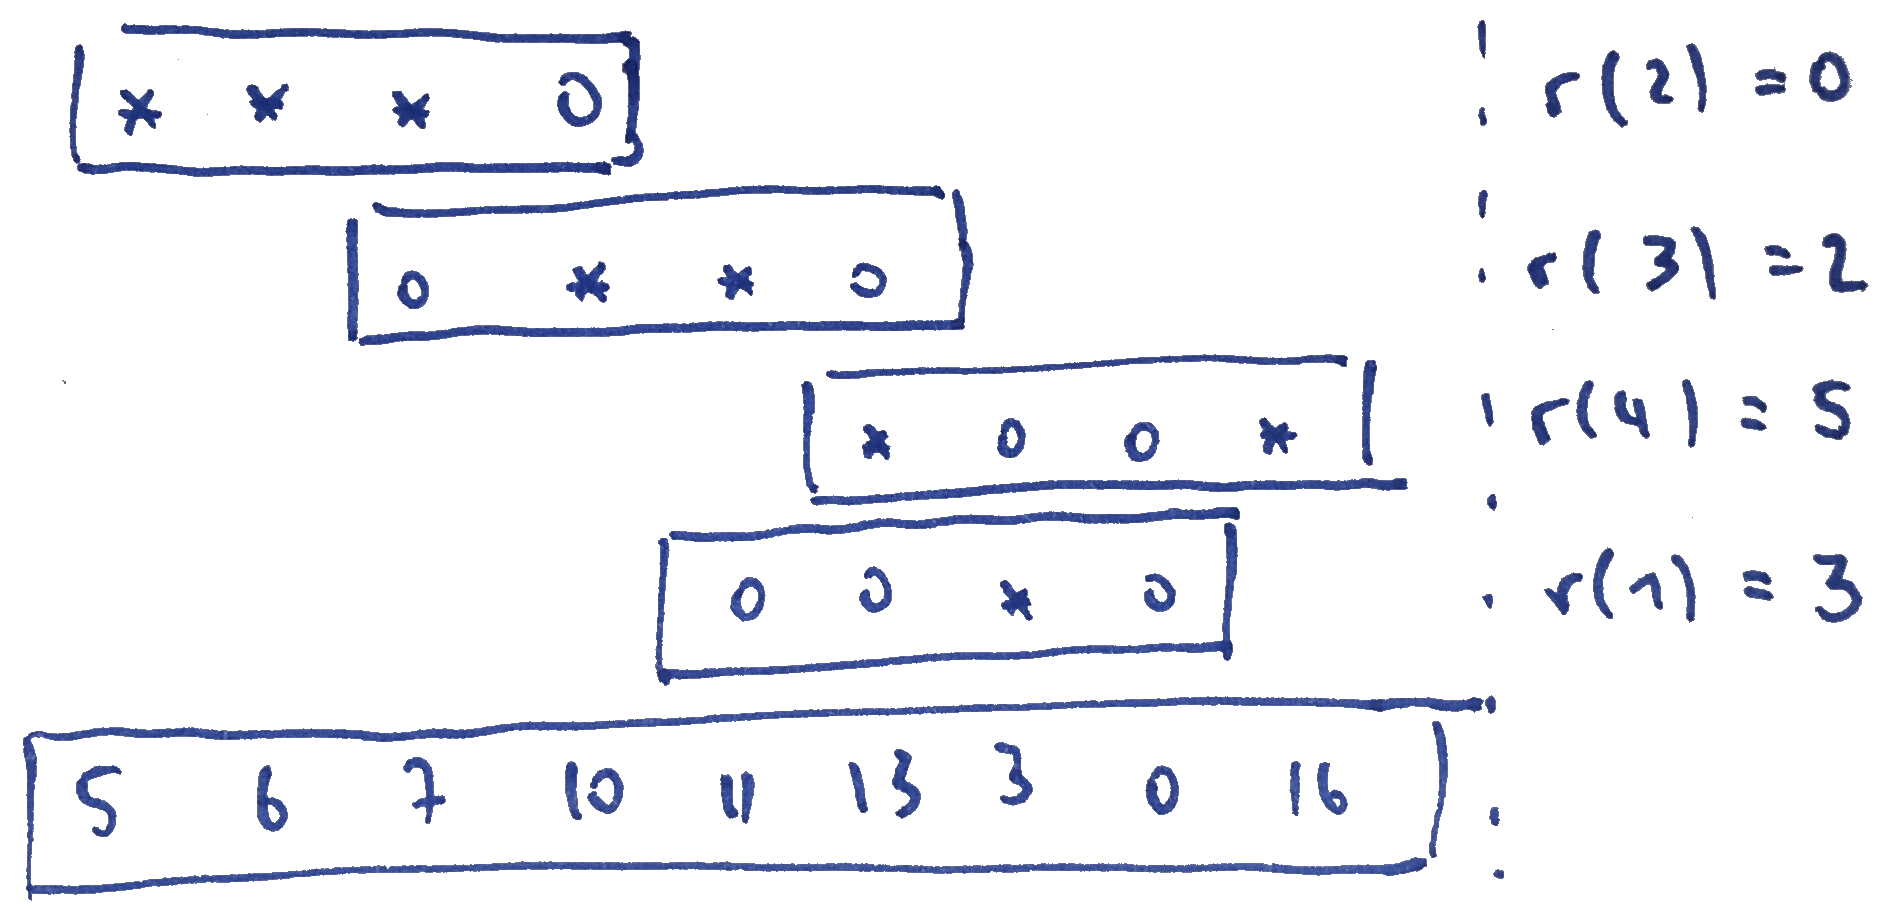
\includegraphics[width=0.5\textwidth]{topic/collapse}
	\caption{Rows of a table collapsed into a one-dimensional array. \label{fig:row_disp}}
\end{wrapfigure}

The compression of such a table $A$ happens in two steps.
Since we consider the static case of table storage, we know all entries before any lookup is performed and we can first insert all $n$ entries into $A$.
Now, we transform $A$ into a one-dimensional array $C$ by mapping every position in $A$ to an index of $C$.
The idea is that we overlap the rows of $A$ so that null entries from previous rows are overwritten by non-null entries of later rows. See Figure~\ref{fig:row_disp}.
Note that the displacement for each row is not calculated in the order in which they appear in the table.
The reason is the following:
Our goal is to minimize the size of $C$.
However, finding the optimal row displacements for a given table is an NP-complete problem.
Instead, we use a heuristic that gives good results for common use cases.
The rows are first sorted by the number of zeroes they contain.
Then we displace every row stepwise until no overlaps with previous rows occur.



\section*{RDI Compression}
\begin{frame}{RDI Compression}
	\centering
	\resizebox{!}{0.75\textheight}{
		\begin{tikzpicture}[align=center, node distance=0.5cm and 1cm]
			\matrix (ri) [%
				matrix of nodes,
				draw = none,
				row sep = 0.7em,
				column sep = 0em
			]
			{
				\alert<6-8,10>{0}    \\
				\alert<6-8,10>{0}    \\
				\alert<6-8>{$\s$} \\
				\alert<7-8>{$\s$} \\
				\alert<7-8,10>{0}     \\
				\alert<7-8>{$\s$} \\
				\alert<8,10>{0}      \\
				\alert<8>{$\s$} \\
				\alert<8,10>{0}    \\
				\alert<10>{0}     \\
				\alert<10>{0}     \\
				\alert<10>{0}     \\
			};
			\node[draw, fit = (ri-1-1) (ri-12-1)] (ri-fit) {};
			\node[above = of ri-1-1] (rilabel) {$r_i$};
			
			\foreach \n in {1,...,12} {
				\node[font=\scriptsize, left = 0.5cm of ri-\n-1 ] {\n};
			}
			
			\visible<2->{
				\matrix (R) [%
					matrix of nodes,
					draw = none,
					row sep = 0.7em,
					column sep = 0em,
					right = of ri
				]
				{
					$r_3$ \\ $r_4$ \\ \alert<16>{$r_6$} \\ $r_8$ \\
				};
				\node[draw, fit = (R-1-1) (R-4-1)] (r-fit) {};
				\node[above = of R-1-1] (Rlabel) {$R$};
				
				\foreach \n in {1,...,4} {
					\node[font=\scriptsize, left = 0.25cm of R-\n-1 ] {\n};
				}
			}
			
			
			\visible<3->{
				\node[draw, fit = (ri-4-1) (ri-6-1)] (c) {};
				\node[draw, fit = (ri-10-1) (ri-12-1)] (d) {};
			}
			
			
			\visible<4->{
				\matrix (D) [%
					matrix of nodes,
					draw = none,
					row sep = 0.7em,
					column sep = 0em,
					right = of R
				]
				{
					\alert<5>{0} \\
					\alert<6,15>{1} \\
					\alert<7>{3} \\
					\alert<8>{4} \\
				};
				\node[draw, fit = (D-1-1) (D-4-1)] (D-fit) {};
				\node[above = of D-1-1] (Dlabel) {$D$};
			}
			
			\visible<6>{
				\draw[edge, red] (D-2-1.west) to[out=180, in=0] (R-1-1.east);
			}
				
			\visible<7>{
				\draw[edge, red] (D-3-1.west) to (R-3-1.east);
			}
				
			\visible<8>{
				\draw[edge, red] (D-4-1.west) to (R-4-1.east);
			}
			
			
			\visible<9->{
				\matrix (I) [%
					matrix of nodes,
					draw = none,
					row sep = 0.7em,
					column sep = 0em,
					right = of D
				]
				{
					\alert<10>{0} \\
					\alert<10>{0} \\
					\alert<11>{1} \\
					\alert<12>{1} \\
					\alert<10>{0} \\
					\alert<12,15>{2} \\
					\alert<10>{0} \\
					\alert<13>{1} \\
					\alert<10>{0} \\
					\alert<10>{0} \\
					\alert<10>{0} \\
					\alert<10>{0} \\
				};
				
				\node[draw, fit = (I-1-1) (I-12-1)] (i-fit) {};
				\node[above = of I-1-1] (Ilabel) {$I$};
				
				
				
				\node[draw, fit = (I-4-1) (I-6-1)] (a) {};
				\node[draw, fit = (I-10-1) (I-12-1)] (b) {};
			}
			
			
			\visible<14->{
				\node[right = 1cm of I-6-1] (lu6) {6 (in section 2)};
				\draw[edge] (lu6.west) to (I-6-1.east);
			}
			
		\end{tikzpicture}
	}
\end{frame}

\begin{frame}{RDI Compression}
	\begin{itemize}[<+->]
		\itemspacing{20pt}
		\item Values in $I$ are in $\O{\log \log n}$
		\item Pack multiple small values into one
		\item Reduces required storage for $I$
		\item Achieves overall compression of row displacements
	\end{itemize}
\end{frame}



\section*{Conclusion}
We used row and column displacements to create a storage scheme that reduces the number of null entries that have to be stored for a not too sparse square table.
Using row displacement directories, the storage for the row displacements can be reduced even more.
By using the internal structure of the trie data structure, we finally get a storage scheme that is good for all tables.
\newpage


\bibliographystyle{abbrv}
\bibliography{literature}

\end{document}
